\chapter{Design}

\subsection{Database}
\begin{figure}[htbp]
	\centering
	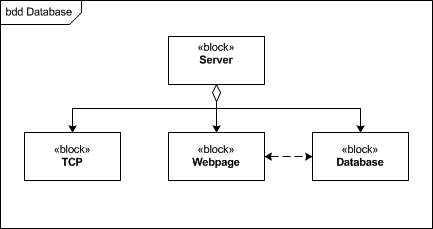
\includegraphics[width=0.6\textwidth]{billeder/bdd_server}
	\caption{BDD server}
	\label{fig:bdd_server}
\end{figure}

Databasen er en server som har de 3 underblokke TCP, Database og Web-page som illustreret på figur \ref{fig:bdd_server}

TCP er en dataforbindelse (Transmission Control Protocol). Denne protokol er benyttes til at sende data fra KI til serveren. Severen vil modtage data og lagere dette i en midlertidig backup fil. TCP-forbindelsen er kodet i C++.
For TCP-forbindelsen benyttes TCP - protocollen som tilbyder sikker data overførelse fra BROS.
Databasen er en mySQL database som frit kan downloades og installeres på en linux maskine. Man kan her vælge at installere en server del og en client del. Server delen er den del som i projektet benyttes da denne giver mulighed for at skrive til databasen samtidig med at man fra f.eks. en web-page kan tilgå og aflæse de data som er lageret i den. mySQL kan tilgås direkte fra terminalen og giver mulighed for forskellige opsætninger af databaser og tabeller samt forskellige bruger rettigheder.
Web-pagen er udviklet i php som giver gode muligheder for kommunikation til og fra mySQL databasen. Web-pagen er implementeret ved hjælp af en apache server som er en web server. Web-pagen har en general information omkring BROS og et login til at tilgå databasen. Den web baserede database loader mySQL databasen og fremviser denne grafisk for brugeren.

